\subsection{Processos de Negócio e Modelação Dimensional}

A modelação do processo ETL é complementada pela criação de diagramas BPMN que permitem representar de forma clara e sistemática o fluxo de atividades envolvidas na preparação dos dados que irão alimentar o Data Warehouse. Estes diagramas facilitam a compreensão das várias fases do processo, permitindo identificar dependências e contribuem para a deteção de possíveis pontos de melhoria na execução das tarefas.

Existem três níveis de diagramas BPMN que representam a aplicação do processo ETL, sendo eles: nível do processo; nível padrão e nível da tarefa. Sendo que, no âmbito deste projeto, não foi necessário a especificação dos diagramas ao nível da tarefa, como também não foram descritos de forma individual todos os processos ao nível padrão, visto que são todos bastante semelhantes entre si 

\subsection{Visão Global do Processo}
A Figura \ref{fig:bpmnprocesso} ilustra a arquitetura macroscópica do fluxo ETL, modelada através de um diagrama BPMN ao nível do processo. Esta representação de alto nível oferece uma visão abrangente das etapas fundamentais, desde o carregamento das tabelas de dimensão até às tabelas de factos utilizadas pelo \textit{Data Warehouse}

\begin{figure}[h!]
	\centering
	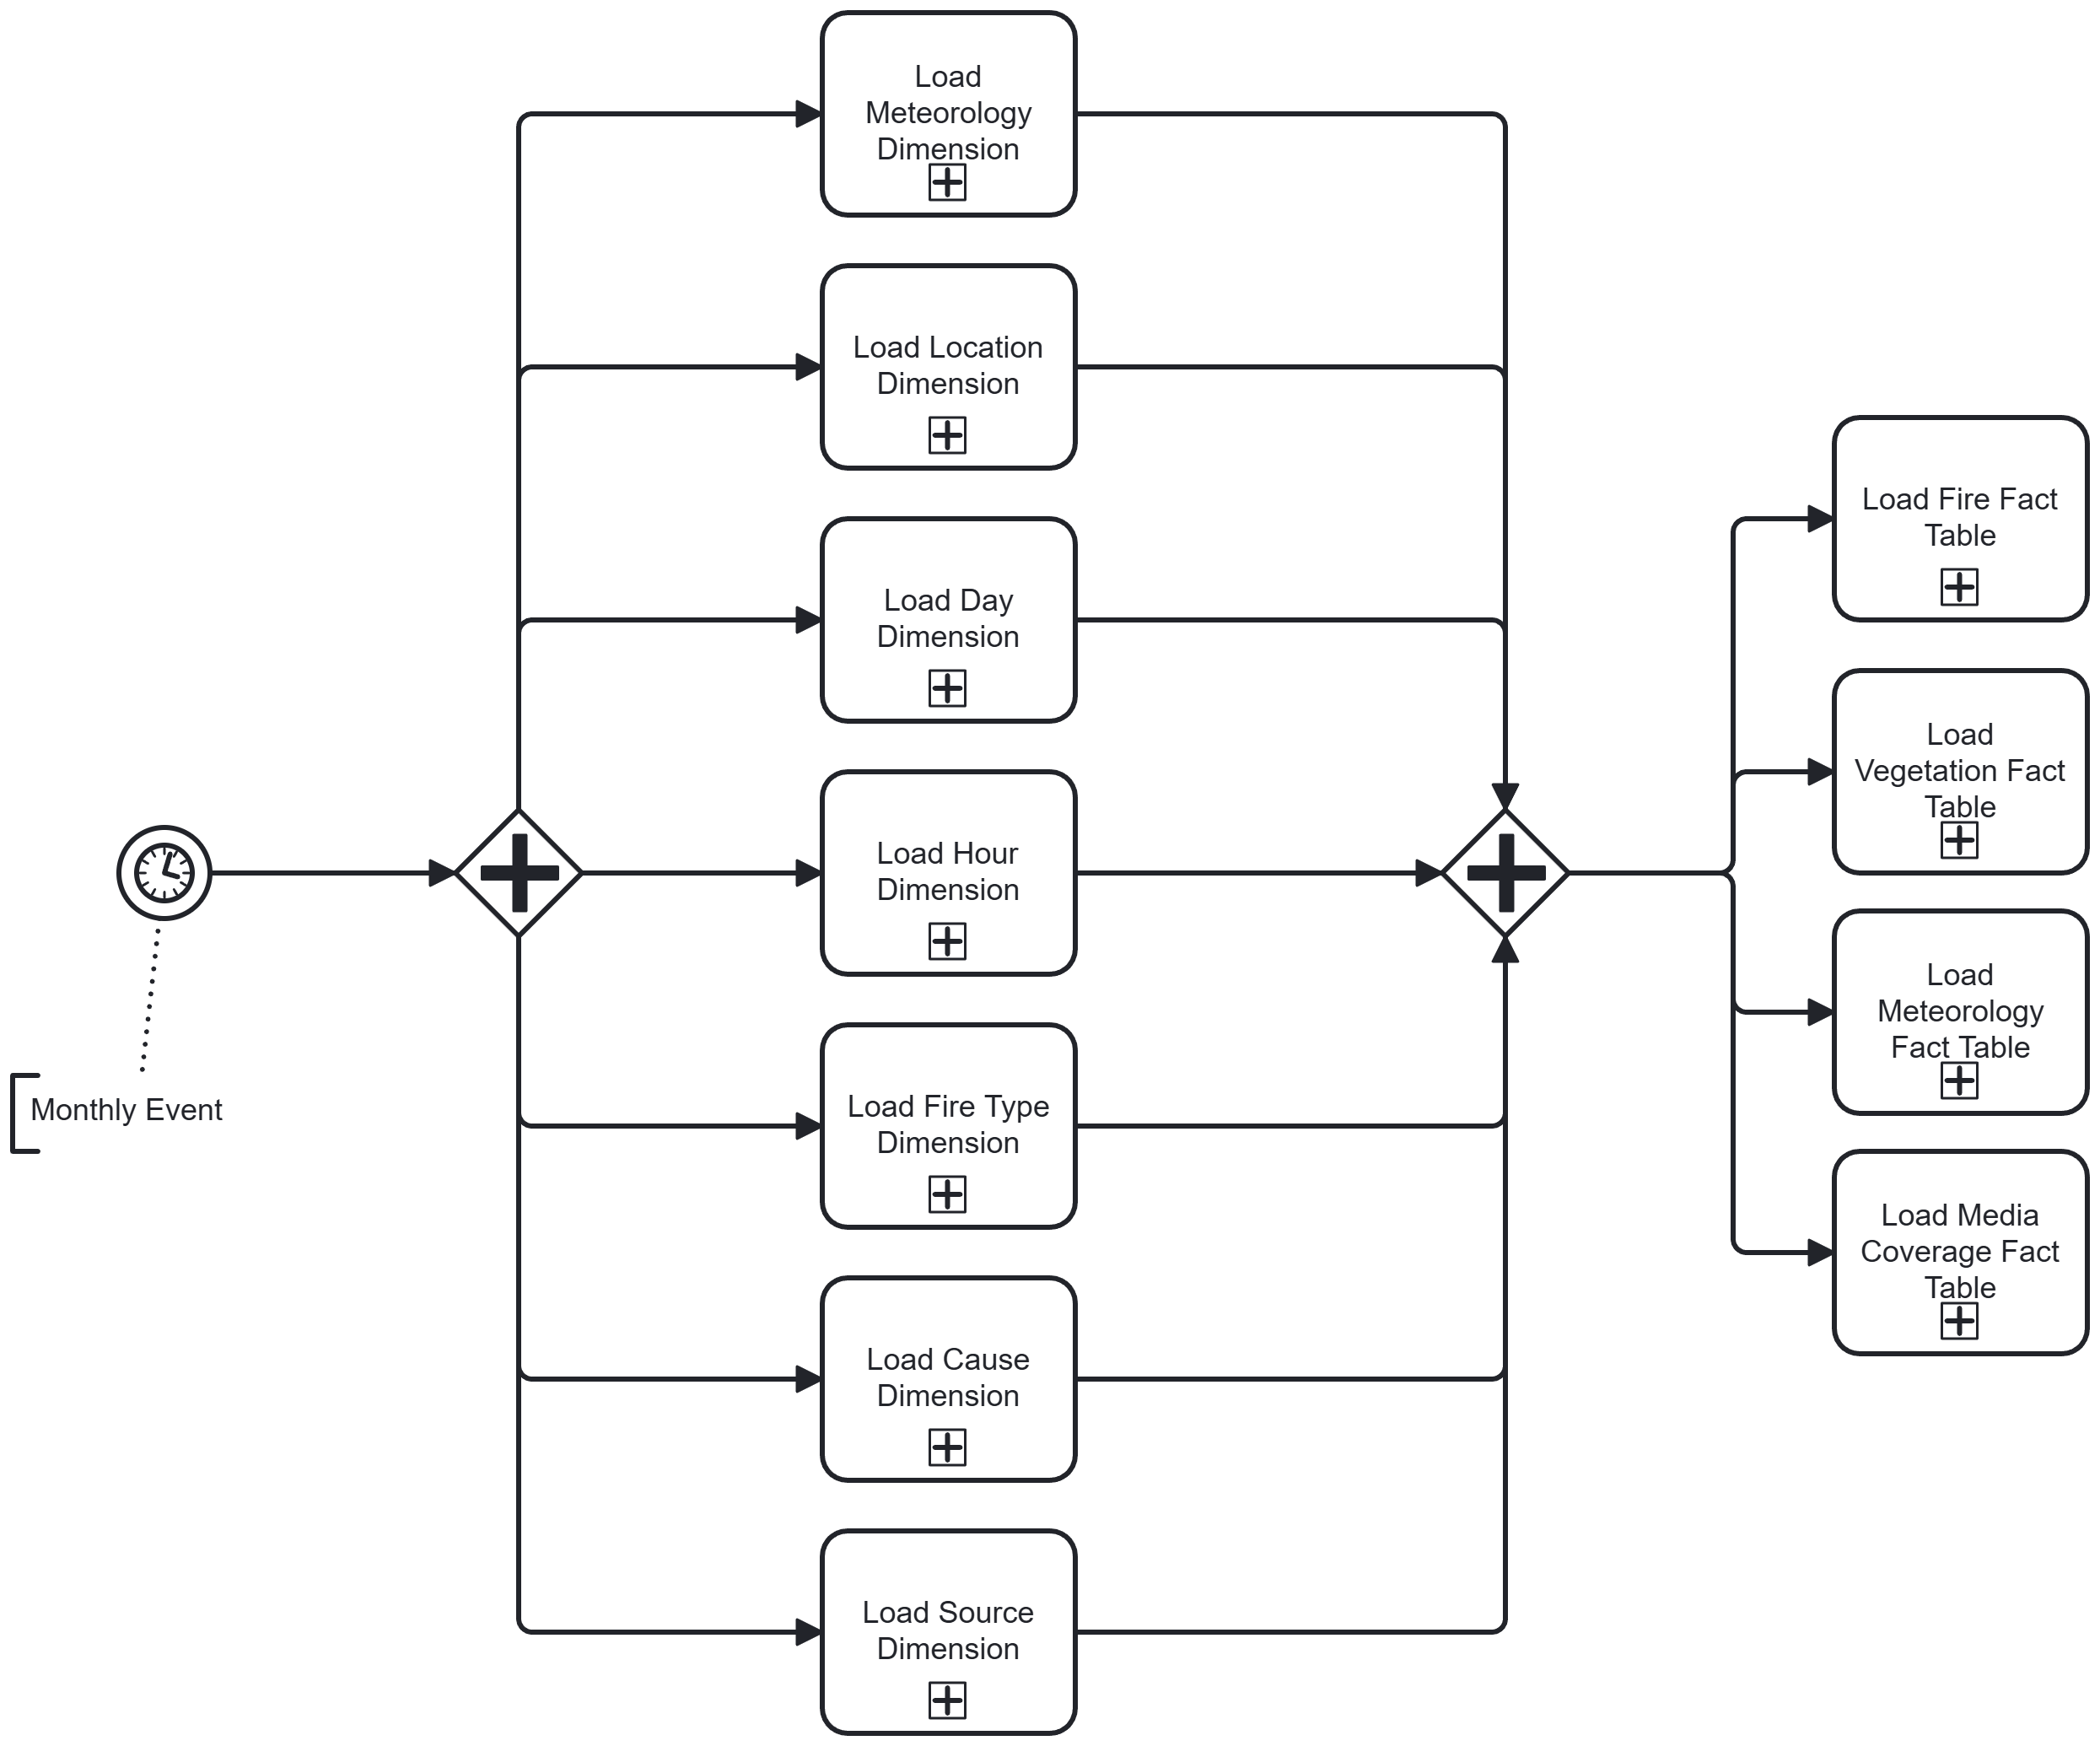
\includegraphics[width=1\linewidth]{imagens/BPMN_Processo}
	\caption{Diagrama BPMN ao nível do processo}
	\label{fig:bpmnprocesso}
\end{figure}



\subsection{Detalhe de Atividades Específicas}
Algumas partes do processo ETL são representadas por diagramas BPMN ao nível padrão. Estes diagramas permitem aprofundar tarefas que exigem uma descrição mais granular, como procedimentos de validação, mecanismos de controlo de qualidade ou etapas específicas de transformação e enriquecimento dos dados.

Abaixo, detalham-se os fluxos específicos para o carregamento das principais dimensões e da tabela de factos central.

\subsubsection{Carregamento da Dimensão Tipo de Incêndio}
Este processo (Figura \ref{fig:bpmnprocessoloaddaydimension}) foca-se na classificação das ocorrências. O fluxo garante a normalização das categorias de incêndio (ex: Agrícola, Florestal, Queimada) e a gestão de novos tipos que possam surgir nos dados de origem, assegurando a consistência na categorização das ocorrências.

\begin{figure}[htbp]
	\centering
	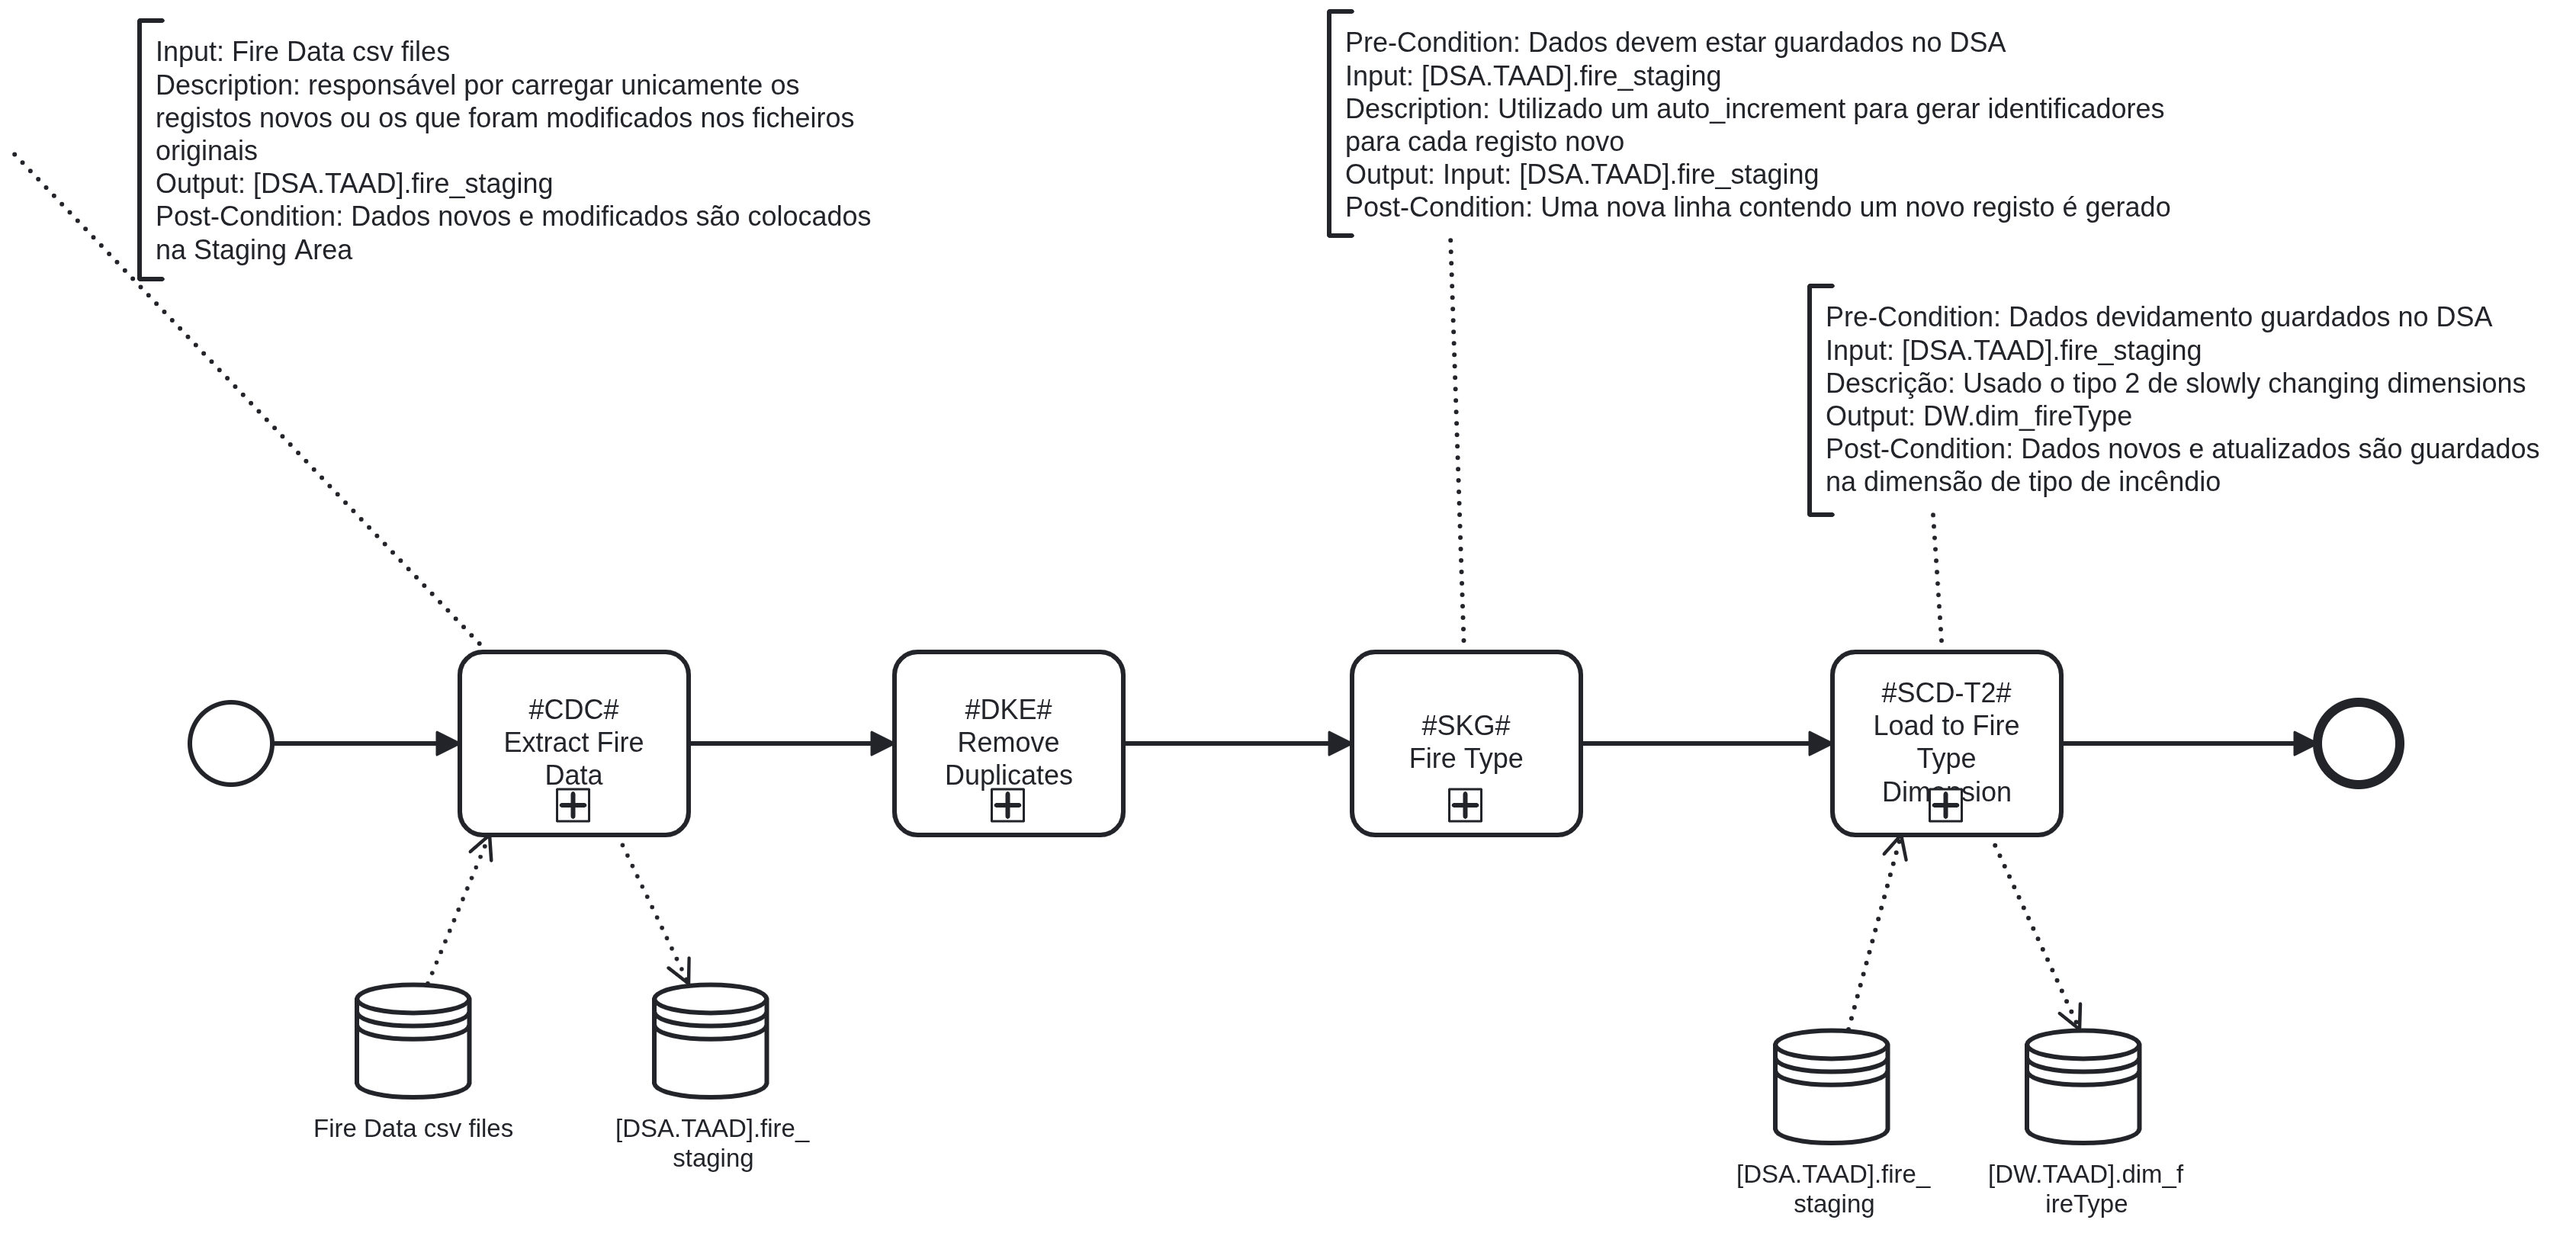
\includegraphics[width=1\linewidth]{imagens/BPMN_Processo_Load_Fire_Type_Dimension}
	\caption{Diagrama BPMN nível padrão para a dimensão Tipo de Incêndio}
	\label{fig:bpmnprocessoloadfiretypedimension}
\end{figure}

\subsubsection{Carregamento da Dimensão Tempo (Dia)}
A dimensão temporal é crítica para a análise de sazonalidade. O processo ilustrado na Figura \ref{fig:bpmnprocessoloaddaydimension} é responsável por gerar e validar os registos diários, permitindo a posterior agregação de factos por dia, mês, ano ou estação.

\begin{figure}[htbp]
	\centering
	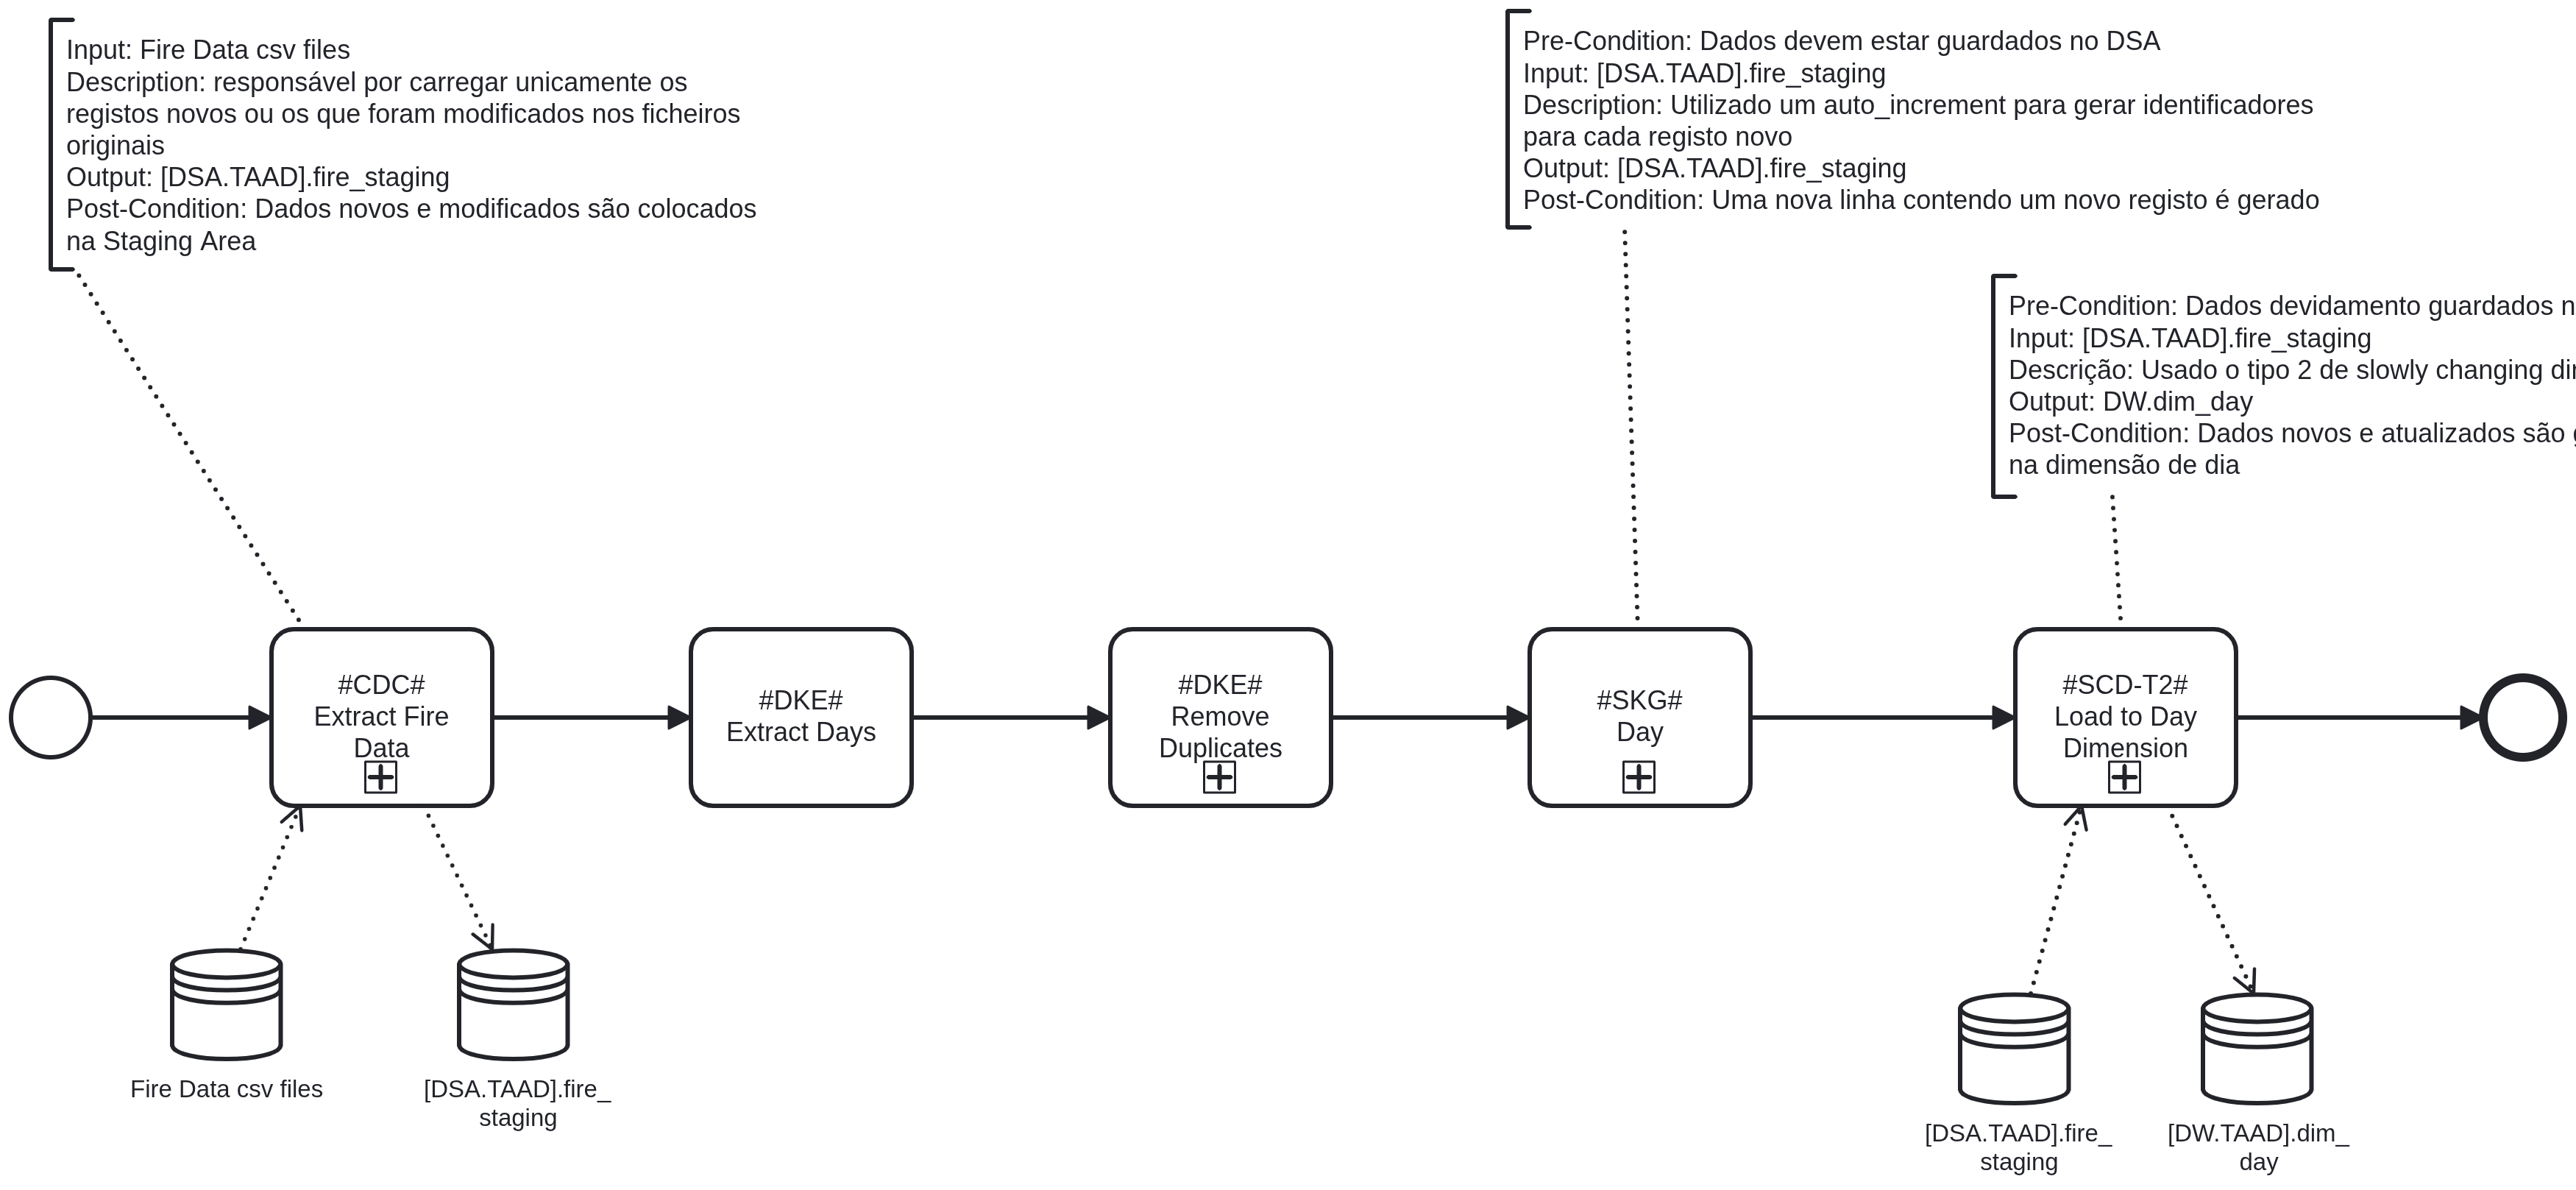
\includegraphics[width=1\linewidth]{imagens/BPMN_Processo_Load_Day_Dimension}
	\caption{Diagrama BPMN nível padrão para a dimensão Dia}
	\label{fig:bpmnprocessoloaddaydimension}
\end{figure}

\subsubsection{Carregamento da Dimensão Localização}
Dado o carácter geográfico do projeto, o carregamento da dimensão de localização exige validações rigorosas. O fluxo trata da hierarquia espacial (Distrito > Concelho > Freguesia), validando as coordenadas e garantindo a integridade referencial das áreas administrativas afetadas. % TODO eu não fali isto

\begin{figure}[htbp]
	\centering
	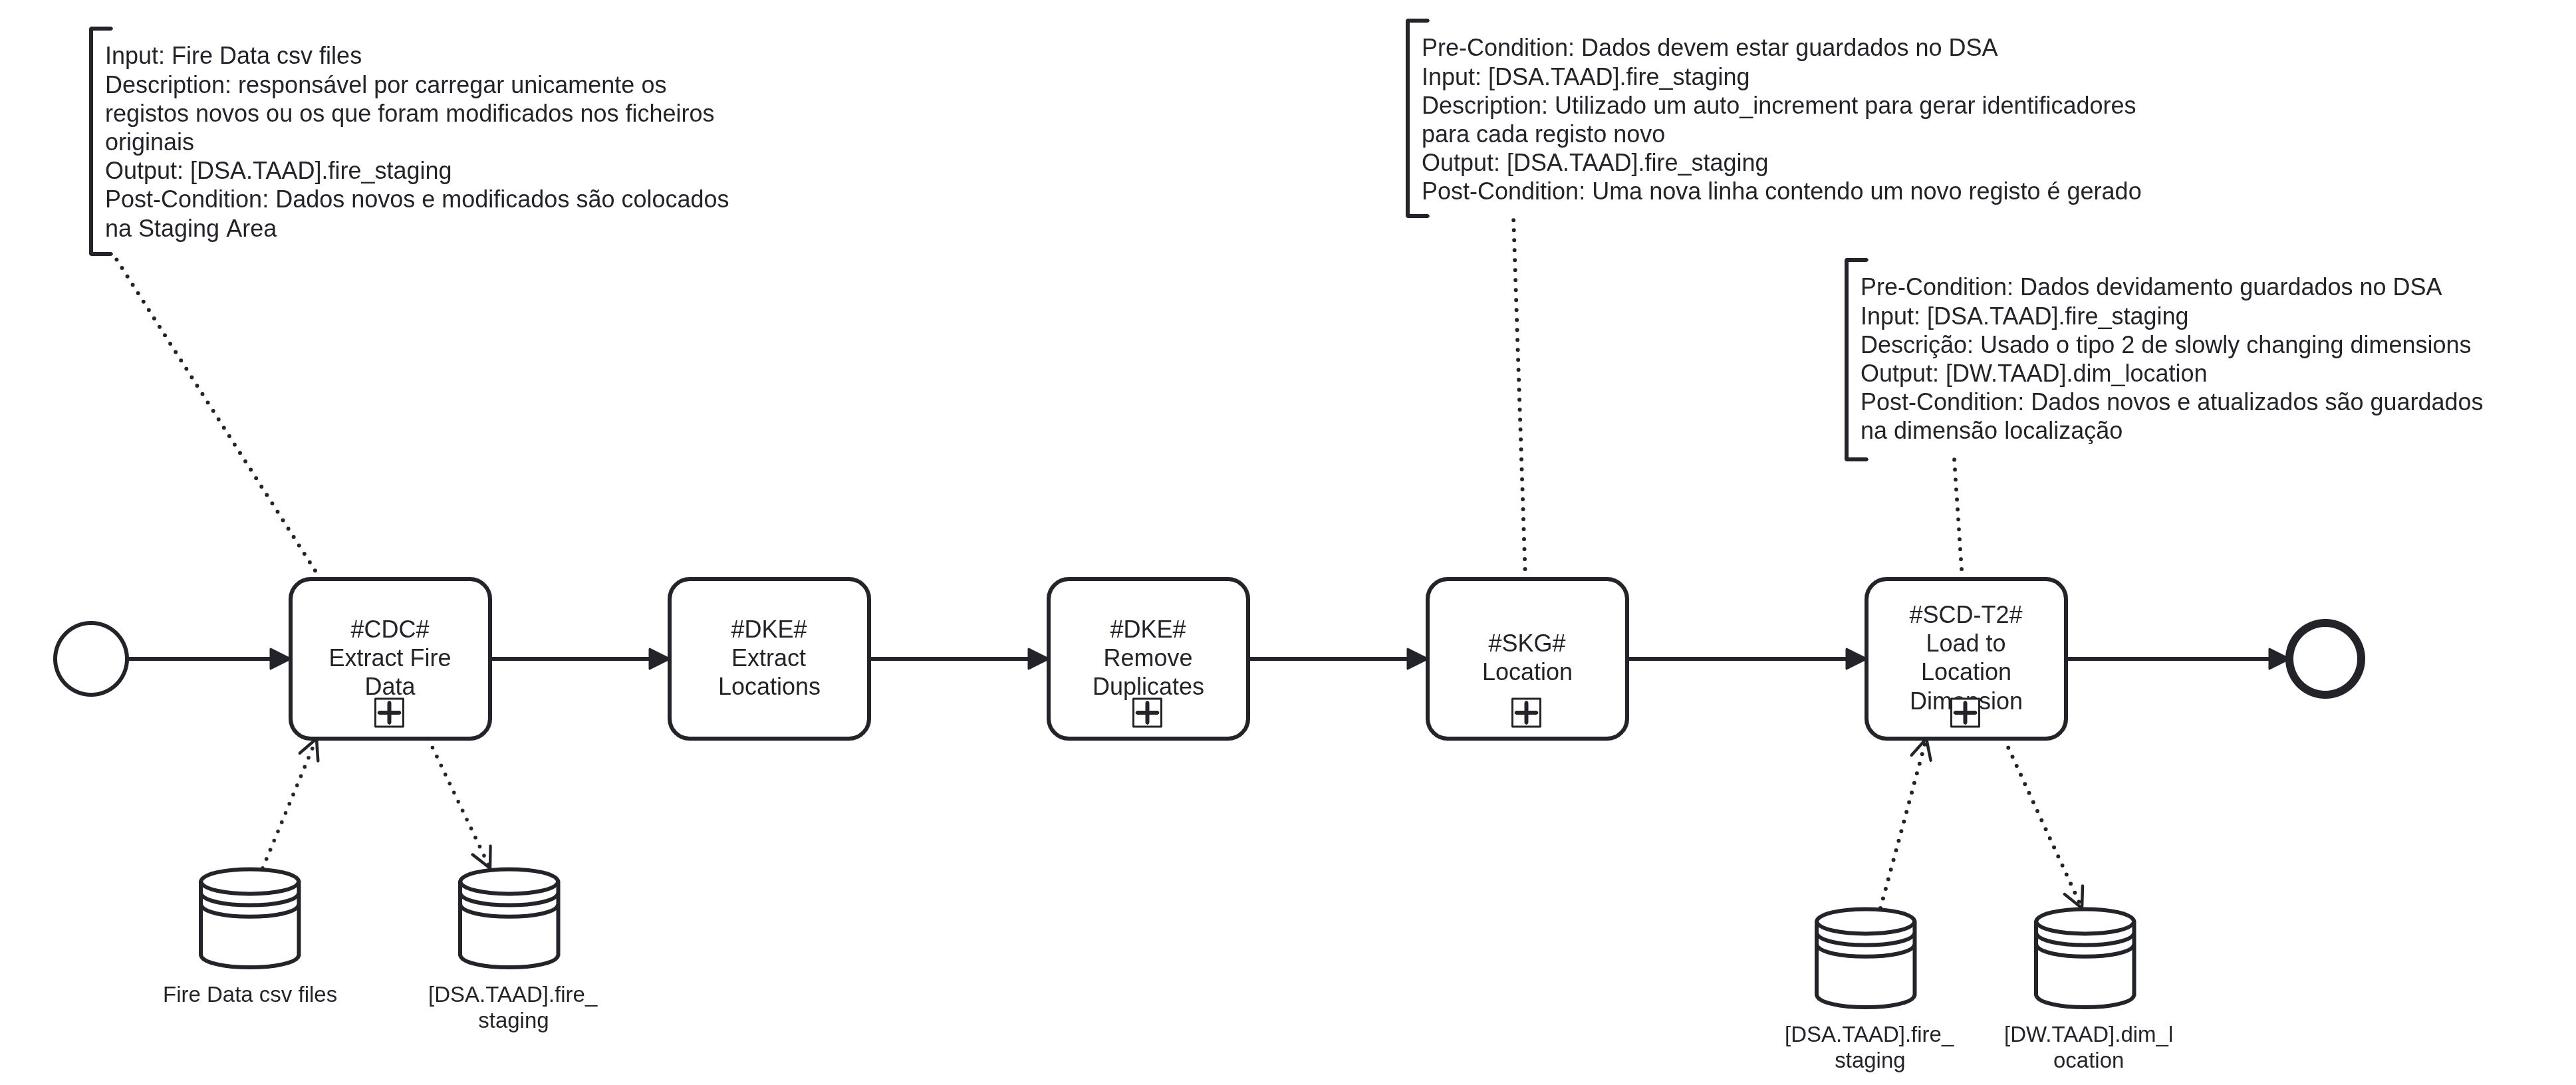
\includegraphics[width=1.0\linewidth]{imagens/BPMN_Processo_Load_Location_Dimension}
	\caption{Diagrama BPMN nível padrão para a dimensão de Localização}
	\label{fig:bpmnprocessoloadlocationdimension}
\end{figure}

\subsubsection{Carregamento da Tabela de Factos de Incêndio}
Este é o processo central do sistema, onde as métricas (área ardida, duração) são misturadas com as chaves das dimensões anteriormente carregadas. O diagrama da Figura \ref{fig:bpmnprocessoloadfirefacttable} demonstra a lógica de obtenção das chaves substitutas (\textit{surrogate keys}) e o cálculo de medidas derivadas antes da inserção final no Data Warehouse.

\begin{figure}[htbp]
	\centering
	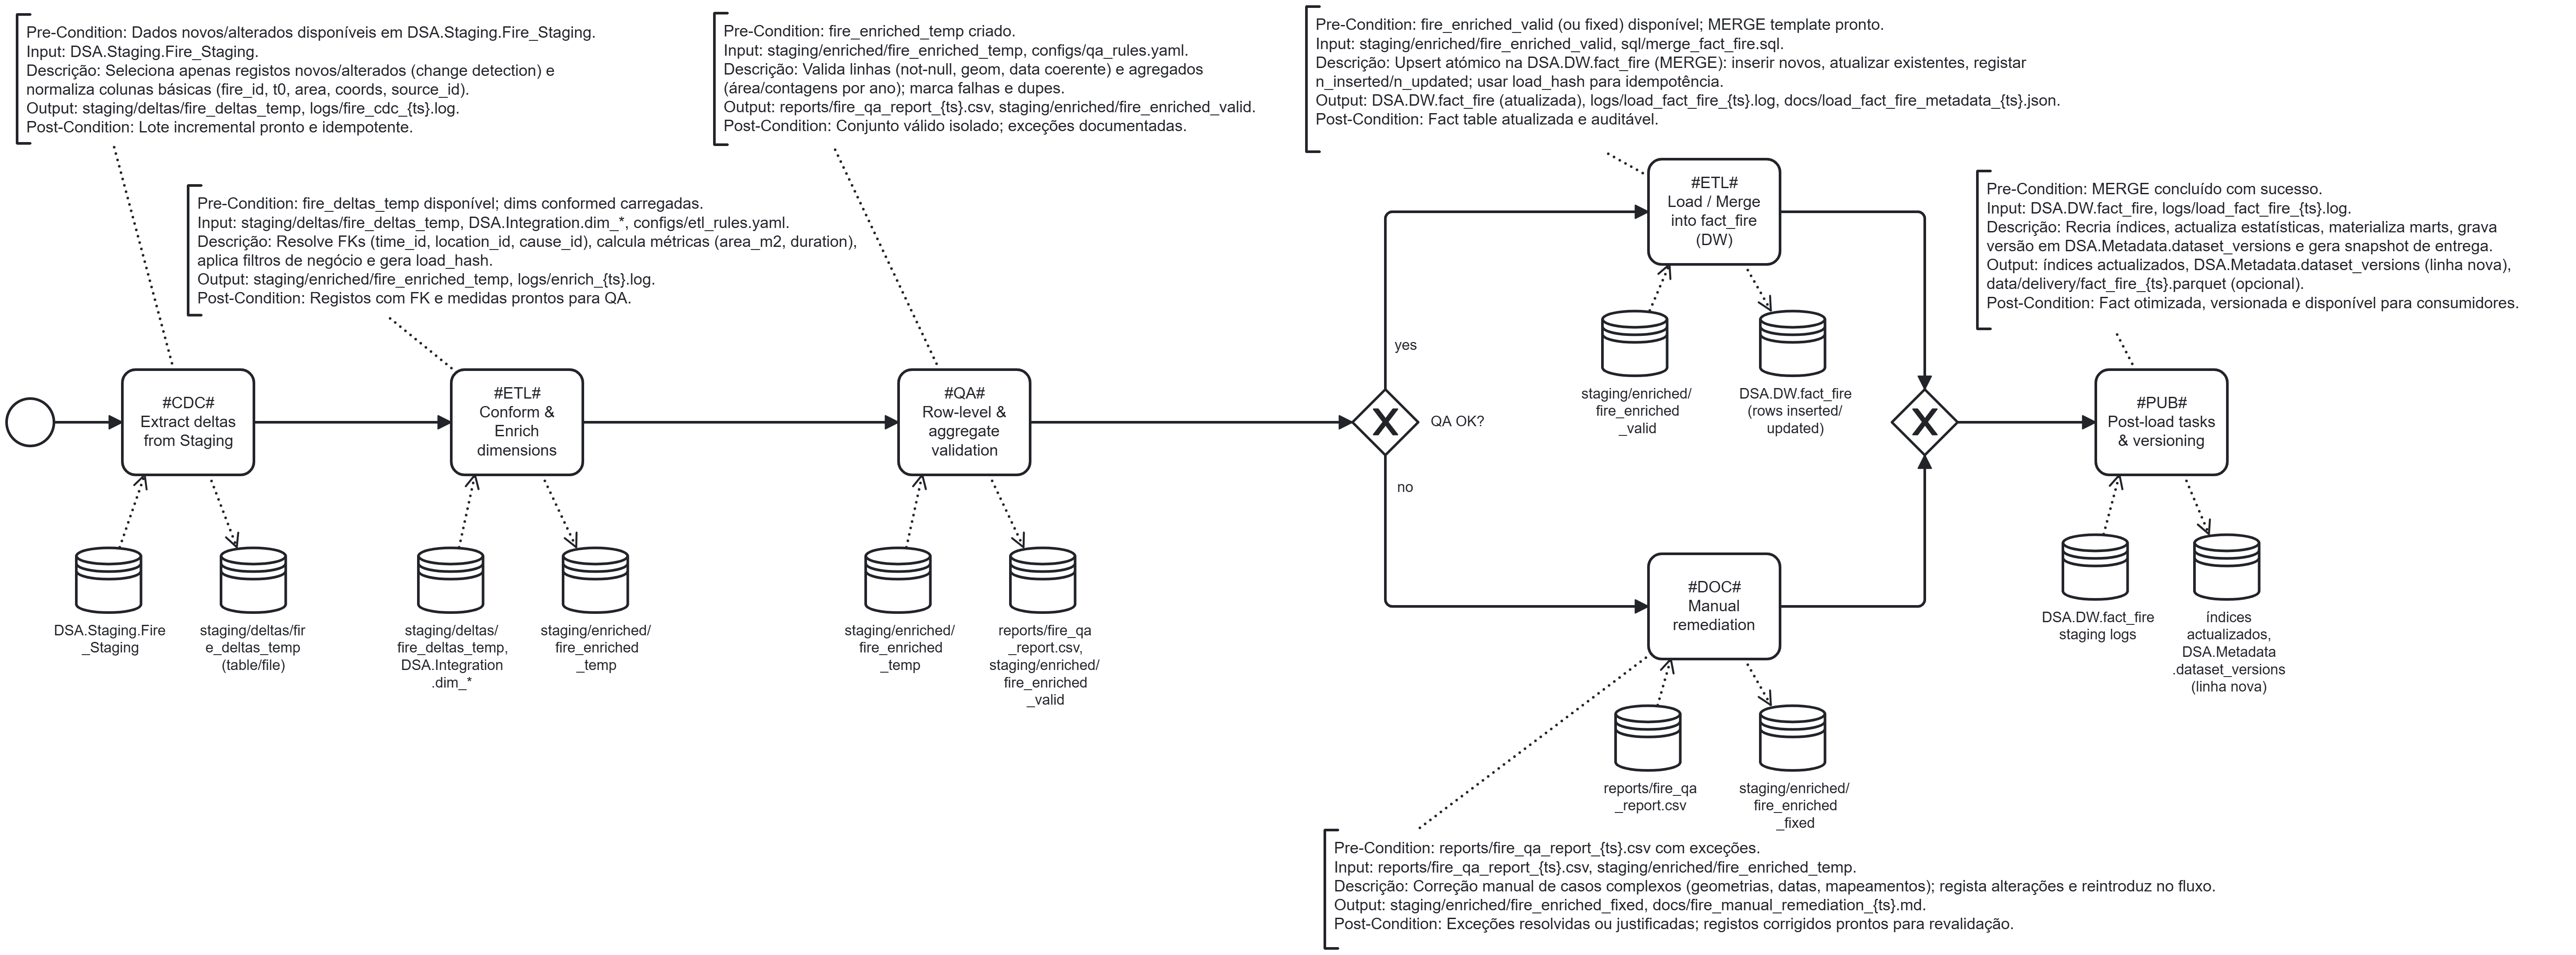
\includegraphics[width=1\linewidth]{imagens/BPMN_Processo_Load_Fire_Fact_Table}
	\caption{Diagrama BPMN nível padrão para a tabela de factos de Incêndio}
	\label{fig:bpmnprocessoloadfirefacttable}
\end{figure}